Die Parameter werden nach dem physikalischen Ersatzschaltbild des
Bipolartransistors ohne parasitäre Kapazitäten bestimmt. Bei der
Kleinsignalanalyse werden alle Kapazitäten sowie Spannungsquellen als
Kurzschlüsse behandelt.

\subsubsection{Emitterschaltung}

\begin{figure}[H]
  \begin{center}
    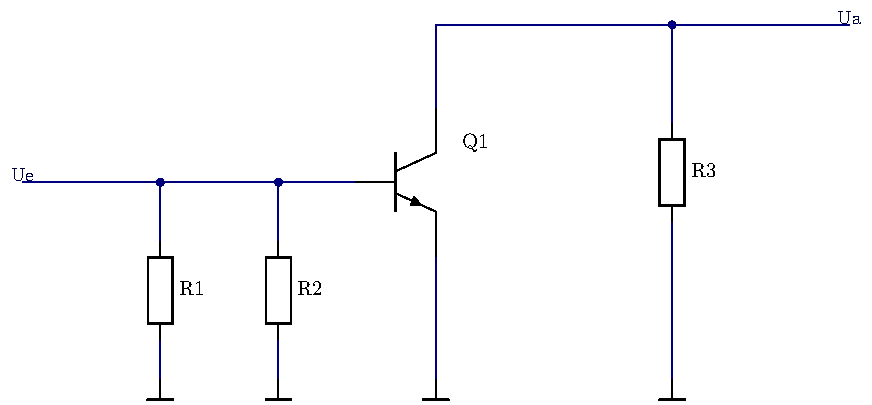
\includegraphics[width=0.618\textwidth]{circuits/commonEmitter_ESB1.pdf}
  \end{center}
  \caption{Kleinsignalersatzschaltbild der Emitterschaltung (Abb. 3)}
\end{figure}

\begin{figure}[H]
  \begin{center}
    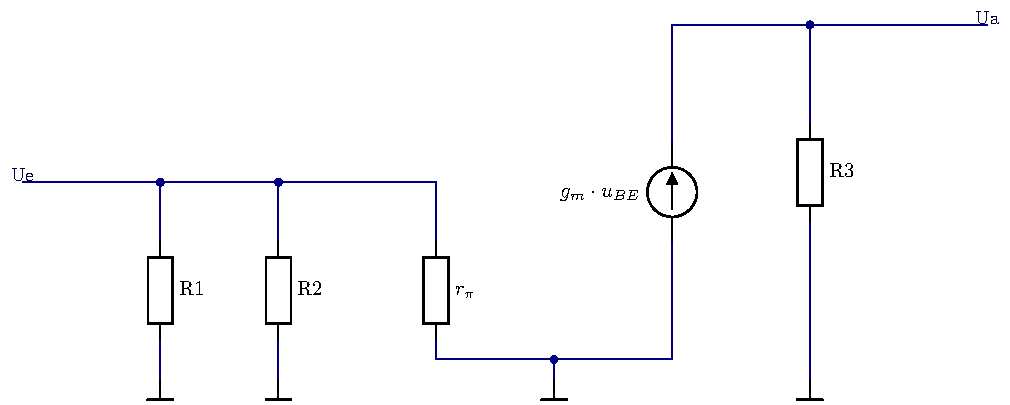
\includegraphics[width=0.618\textwidth]{circuits/commonEmitter_ESB2.pdf}
  \end{center}
  \caption{ESB Abb. 6, Transistor durch phys. ESB ersetzt}
\end{figure}

\noindent Eingangswiderstand:
\[r_e = \frac{U_e}{I_e}|_{U_a = 0} = R_1 // R_2 // r_\pi\]
\noindent Ausgangswiderstand:
\[r_a = \frac{U_a}{I_a}|_{U_e = 0} = r_0 // R_3 \]
\noindent Spannungsverstärkung:
\[V_u = \frac{U_a}{U_e}\]
\begin{gather*}
  U_2 = g_m \cdot u_{BE} \cdot (r_0 // R_3) = g_m \cdot U_1 \cdot (r_0 // R_3)\\
  V_u = g_m \cdot (r_0 // R_3)
\end{gather*}

\noindent Stromverstärkung:
\[V_i = \frac{I_a}{I_e}\]
\[\]

\noindent Leistungsverstärkung:

\noindent Leistungsverstärkung:

%%%%%%%%%%%%%%%%%%%%%%%%%%%%%%%%%%%%%%%%%
\subsubsection{Kollektorschaltung}
\begin{figure}[H]
  \begin{center}
    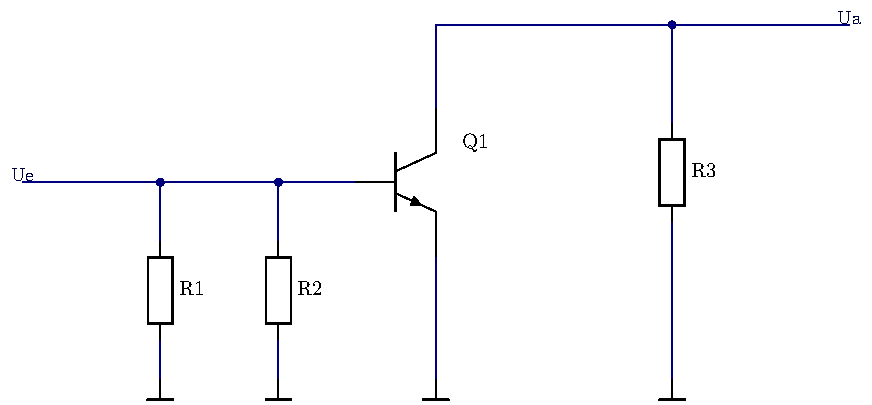
\includegraphics[width=0.618\textwidth]{circuits/commonEmitter_ESB1.pdf}
  \end{center}
  \caption{Kleinsignalersatzschaltbild der Kollektorschaltung (Abb. 4)}
\end{figure}

\begin{figure}[H]
  \begin{center}
   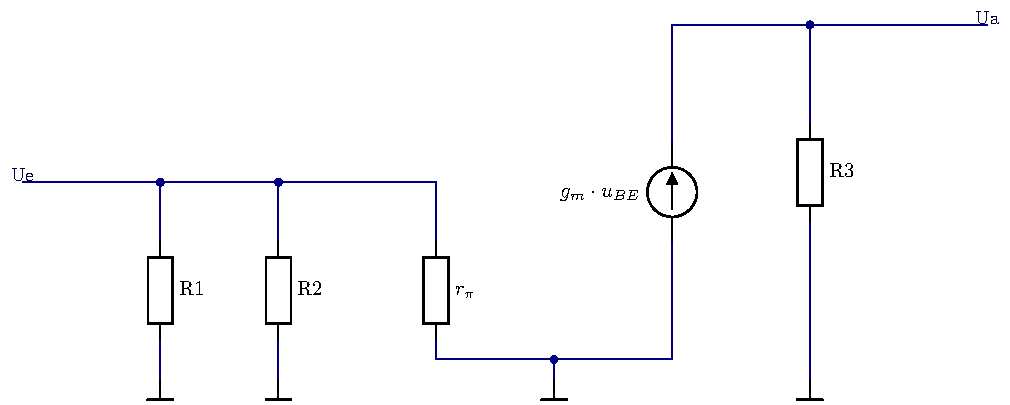
\includegraphics[width=0.618\textwidth]{circuits/commonEmitter_ESB2.pdf}
  \end{center}
  \caption{ESB Abb. 8, Transistor durch phys. ESB ersetzt}
\end{figure}


%%%%%%%%%%%%%%%%%%%%%%%%%%%%%%%%%%%%%%%%%
\subsubsection{Basisschaltung}
\begin{figure}[H]
  \begin{center}
    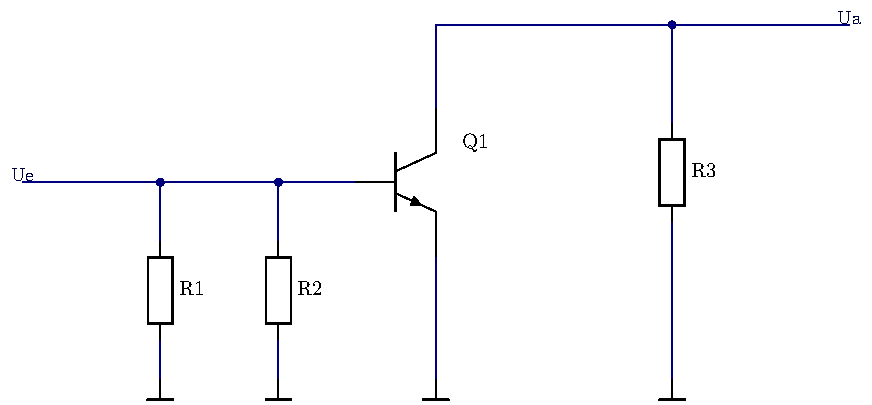
\includegraphics[width=0.618\textwidth]{circuits/commonEmitter_ESB1.pdf}
  \end{center}
  \caption{Kleinsignalersatzschaltbild der Basisschaltung (Abb. 5)}
\end{figure}

\begin{figure}[H]
  \begin{center}
    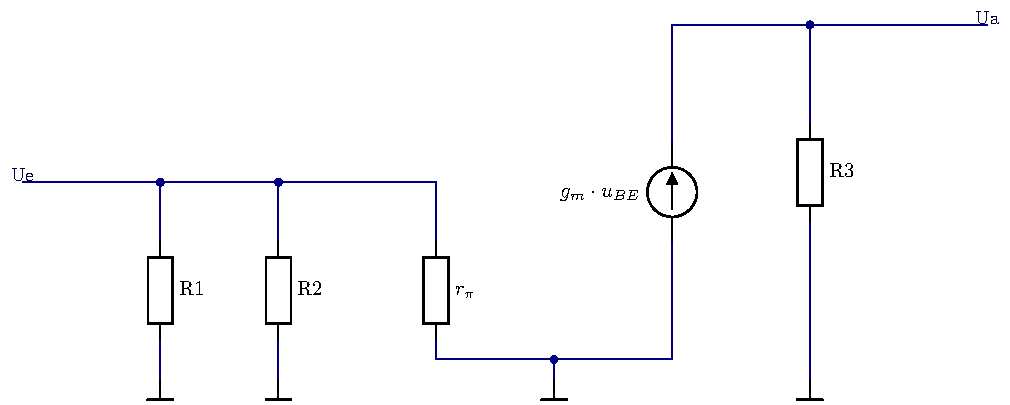
\includegraphics[width=0.618\textwidth]{circuits/commonEmitter_ESB2.pdf}
  \end{center}
  \caption{ESB Abb. 10, Transistor durch phys. ESB ersetzt}
\end{figure}


